\documentclass[11pt]{article}
\usepackage[a4paper,margin=2.3cm]{geometry}
\usepackage[T1]{fontenc}
\usepackage[utf8]{inputenc}
\usepackage{lmodern}
\usepackage{amsmath,amssymb}
\usepackage{booktabs}
\usepackage{multirow}
\usepackage{xcolor}
\usepackage{pgfplots}
\pgfplotsset{compat=1.16}
\usepackage[colorlinks=true,linkcolor=blue!50!black,citecolor=blue!50!black,urlcolor=blue!50!black]{hyperref}

\title{LLM-JEPA on a Crowd-Trained 0.66B Base Model:\\
A Pre-Registered Study on a Shared Tesla T4}
\author{Xavier Callens\\ \small Project HiveMind}
\date{14 November 2026}

\begin{document}
\maketitle

\begin{abstract}
LLM-JEPA adds a joint-embedding predictive term to the next-token objective of language models and reports large gains
on fine-tuning tasks with naturally paired views, including $+11.4$ points at LoRA rank~64 on NL-RX-SYNTH for an
instruction-tuned 1B model. We test whether this transfers to \emph{Crowd-v1}, a 658M-parameter base model trained by
volunteers in the CrowdGPT project, under the constraints of a single Tesla T4 shared with live inference services (at
most 2.7\,GB per experiment, 4.3\,GB of VRAM always left free).
In a pre-registered pilot (LoRA r64, 3 seeds per arm, 1{,}000 test examples), LLM-JEPA brings no gain
($16.90\pm1.06\%$ vs.\ $17.07\pm0.93\%$ exact match) and degrades general held-out loss by $+0.90$ nat. The JEPA term
collapses to $1-\cos\le5\times10^{-4}$. A compute-matched screen of ten pre-registered hypotheses, in the style of
\emph{autoresearch}, shows that stop-gradient, centering and InfoNCE remove the collapse and the damage, and that a
weak JEPA term ($\lambda=0.1$ with loss dropout) combined with stop-gradient or centering approaches, but does not
beat, plain fine-tuning. An inference-only diagnosis locates Crowd-v1's main weakness elsewhere: its gap to
Qwen3-0.6B is $+3.84$ nat on Python code and $+2.44$ on mathematics, against $+0.36$ on its own data. We also find and
fix a held-out evaluation bug that ignored the model's engram table ($+0.35$ nat). Whether the null result is specific to
Crowd-v1 remains open; we describe a ready, pre-registered test that separates model from recipe.
\end{abstract}

\section{Introduction}
Small language models trained by volunteer compute face a token budget far below that of industrial models. LLM-JEPA
\cite{huang2025llmjepa} proposes a way to extract more from data: keep the autoregressive model and its inference
unchanged, but add, during training, a term that asks the final hidden state of one view of a content (e.g.\ a natural
language description) to predict the embedding of another view (e.g.\ the corresponding regular expression). The paper
reports gains on several fine-tuning tasks, with the largest on NL-RX-SYNTH \cite{locascio2016nlrx}.

We study this method for \emph{Crowd-v1}, the 1B-class (658M trunk parameters) model of the CrowdGPT project, trained
by volunteer GPUs with periodic delta aggregation, a scheme close to DiLoCo \cite{douglas2023diloco}. Our constraints
are those of a small open project: a single Tesla T4 that also serves inference, a hard rule to keep 4.3\,GB of VRAM
free, and no budget for larger accelerators. Within those constraints we ask three questions:
(i) what is the real held-out quality of Crowd-v1;
(ii) does LLM-JEPA improve it on a paired-view task, and can it be tuned to;
(iii) where else could Crowd-v1 be improved.
All decisive experiments were pre-registered: protocols and success criteria were written before any result.

\paragraph{Contributions.}
\begin{itemize}
\item An evaluation fix: the held-out loss check of the project ignored the model's engram table, which costs
$0.35$ nat (Section~\ref{sec:e0}).
\item A pre-registered null result for LLM-JEPA on Crowd-v1 with LoRA r64, with a measured collapse of the JEPA term and
a $+0.90$ nat degradation of general loss (Section~\ref{sec:p1}).
\item A compute-matched screen of 10 hypotheses (5 tested) identifying two levers that combine: weak JEPA pressure and
an anti-collapse mechanism (Section~\ref{sec:ar}).
\item A per-domain diagnosis showing that the data mix, not the training objective, is Crowd-v1's main limitation
(Section~\ref{sec:p0}).
\item An open, ready-to-run test of whether the null result is model- or recipe-specific (Section~\ref{sec:disc}).
\end{itemize}

\section{Background}
\paragraph{LLM-JEPA.} Given two views $T$ (text) and $C$ (code) of the same content, LLM-JEPA minimizes
\begin{equation}
\mathcal{L} = \sum_\ell \mathcal{L}_{\text{NTP}}(T, C) + \lambda\, d\big(\mathrm{Pred}(\mathrm{Enc}(T)), \mathrm{Enc}(C)\big),
\qquad d = 1-\cos,
\end{equation}
where $\mathrm{Enc}(x)$ is the last-layer hidden state of the last token of $x$. The predictor reuses the model's own
weights through $k$ appended predictor tokens ($k=0$ is the identity). Following the JEPA line of work
\cite{lecun2022path,assran2023ijepa}, the next-token term is what prevents collapse; the paper reports that dropping it
yields empty outputs. Training cost is about $2\times$; inference is unchanged \cite{huang2025llmjepa}. The reference code
applies no stop-gradient.

\paragraph{Anti-collapse mechanisms.} Joint-embedding methods avoid trivial solutions with asymmetric stop-gradient
\cite{grill2020byol}, contrastive negatives (InfoNCE, \cite{oord2018cpc}) or variance/covariance regularization
\cite{bardes2022vicreg}. Contextual embeddings of language models are also known to be anisotropic
\cite{ethayarajh2019contextual}, which makes a raw cosine between final states easy to drive towards 1.

\paragraph{autoresearch.} \emph{autoresearch} \cite{karpathy2026autoresearch} runs an agent loop over a fixed
evaluation and a fixed wall-clock training budget (5 minutes on an H100), with one change per experiment, kept if the
single metric improves and reverted otherwise.

\section{Setup}
\label{sec:setup}
\paragraph{Model.} \texttt{Vxtzq/Crowd-v1}, revision \texttt{5ac3916} (global step 366): 24 layers, width 1536,
grouped-query attention (16/4 heads), SwiGLU, tied head, 657{,}787{,}392 trunk parameters, plus a bigram \emph{engram}
table of 227{,}865 buckets $\times$ 1536 ($350{,}000{,}640$ parameters) added to the token embedding. Tokenizer: Qwen3
(vocabulary 151{,}669). Reference model: Qwen3-0.6B \cite{qwen3report}, same tokenizer.

\paragraph{Hardware and safety.} One NVIDIA Tesla T4 (15\,GB) that also hosts inference services (about 5.1\,GB) and
other tenants (an ollama model of about 2.4\,GB that loads and unloads). Every experiment runs under a guard that:
\begin{itemize}
\item keeps free VRAM $\ge4300$\,MiB at every step;
\item caps the process at 2.7\,GB;
\item pauses while inference requests are in flight;
\item checkpoints and resumes after aborts;
\item yields to the owner's training jobs.
\end{itemize}

\paragraph{Fine-tuning task.} NL-RX-SYNTH \cite{locascio2016nlrx}: 8{,}000 training pairs; the test set is the first
1{,}000 of 2{,}000 examples; exact string match as in the reference evaluator. Prompt: an instruction, the query and
\texttt{Regex:}; the answer is terminated by \texttt{<|endoftext|>}.

\paragraph{Training.} LoRA \cite{hu2022lora} rank 64 ($\alpha=64$) on all attention and MLP projections; base and engram
frozen in fp16; AdamW, effective batch 16. In the JEPA arm, view 1 is the bare query and view 2 the regex. Both views
are packed in one sequence with a block-causal mask, and the engram bigram input is reset at the start of view 2, so
that view 2 is exactly a separate pass. The next-token loss comes from the normal prompt+answer pass. The embedding is
the final (post-norm) state of each view's last token.

\paragraph{General-loss check.} Mean next-token CE on 12 fixed 2{,}048-token windows of a CrowdGPT chunk not used in
fine-tuning. Base model: 3.194 nat.

\section{Held-out quality of Crowd-v1 (E0)}
\label{sec:e0}
Table~\ref{tab:e0} reports held-out CE on 12 windows per source.
\begin{itemize}
\item The model is healthy: about 3 nat on its own distribution, against 11.93 for a uniform guess.
\item An earlier reading of 8--11 nat came from an older revision measured by a loss check that omitted the engram
table. Omitting it alone costs $+0.35$ nat.
\item fp16, fp32 and bf16 agree to $10^{-3}$ nat on the T4.
\item Cohort training reads 0.78 passes per data sub-slice, and the gap between a recently trained region and a distant
one (0.16 nat) is smaller than Qwen's (0.24): there is no sign of memorization.
\end{itemize}

\begin{table}[t]
\centering
\caption{E0: held-out next-token CE (nat/token), mean (sd) over 12 windows of 2{,}048 tokens.}
\label{tab:e0}
\small
\begin{tabular}{lccc}
\toprule
Model & chunk 1026 @0 & chunk 1026 @200\,MB & wikitext-2 test\\
\midrule
Crowd-v1 + engram (fp16 = fp32 = bf16) & 3.030 (0.355) & 3.194 (0.403) & 4.855 (0.345)\\
Crowd-v1 without engram & 3.376 (0.330) & 3.570 (0.377) & 5.055 (0.308)\\
Qwen3-0.6B & 2.536 (0.300) & 2.776 (0.293) & 3.020 (0.268)\\
\bottomrule
\end{tabular}
\end{table}

\section{Pre-registered pilot: SFT vs.\ SFT + LLM-JEPA (P1)}
\label{sec:p1}
\paragraph{Protocol.} Written before any run:
\begin{itemize}
\item LoRA r64, lr $2\times10^{-4}$ with cosine schedule, 3 epochs (1{,}500 steps), seeds 0--2.
\item JEPA with $\lambda=1$, $k=0$.
\item Criteria:
  \begin{enumerate}
  \item a floor of $\ge5\%$ for SFT seed 0;
  \item success if $\Delta=\overline{\text{JEPA}}-\overline{\text{SFT}}>2\,\sigma_{\text{pooled}}$ and the JEPA general loss
  is $\le$ SFT $+0.05$ nat;
  \item a ``paper-like'' gain if, in addition, $\Delta\ge10$ points.
  \end{enumerate}
\end{itemize}

\paragraph{Results.} Table~\ref{tab:p1} and Figure~\ref{fig:p1}.
\begin{itemize}
\item The floor is met.
\item Criteria 2 and 3 are not: $\Delta=-0.17$ points against a threshold of $1.99$, with paired differences $-0.3$,
$0.0$ and $-0.2$.
\item General loss is $0.90$ nat worse with JEPA.
\item An exploratory $\lambda=4$ run is worse on both counts (15.4\%, 5.012 nat).
\item A secondary prefix-match metric shows no difference either (seeds 1--2: SFT 20.6/19.4, JEPA 19.5/19.8).
\item The JEPA term drops from 0.15 at step 25 to $\le5\times10^{-4}$ in every run.
\item JEPA costs $1.45$--$1.61$\,s per step against $0.71$--$0.83$ for SFT (about $1.9\times$).
\end{itemize}

\begin{table}[t]
\centering
\caption{P1: exact match on 1{,}000 NL-RX-SYNTH test examples and general held-out loss (base 3.194). LoRA r64, lr
$2\times10^{-4}$, 3 epochs.}
\label{tab:p1}
\begin{tabular}{cccccc}
\toprule
Seed & SFT (\%) & JEPA $\lambda{=}1$ (\%) & $\Delta$ & SFT general & JEPA general\\
\midrule
0 & 16.0 & 15.7 & $-0.3$ & 3.789 & 4.605\\
1 & 17.7 & 17.7 & $\phantom{-}0.0$ & 3.719 & 4.652\\
2 & 17.5 & 17.3 & $-0.2$ & 3.830 & 4.770\\
\midrule
mean $\pm$ sd & $17.07\pm0.93$ & $16.90\pm1.06$ & $-0.17$ & 3.779 & 4.676\\
\bottomrule
\end{tabular}
\end{table}

\begin{figure}[t]
\centering
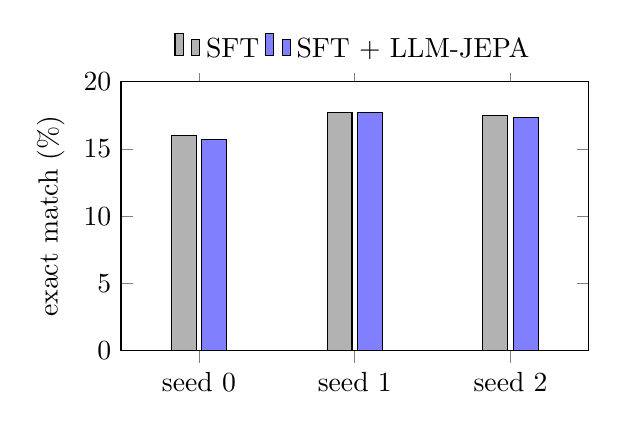
\begin{tikzpicture}
\begin{axis}[ybar, bar width=9pt, width=0.62\linewidth, height=5cm, ymin=0, ymax=20,
  symbolic x coords={seed 0,seed 1,seed 2}, xtick=data, ylabel={exact match (\%)},
  legend style={at={(0.5,1.03)},anchor=south,legend columns=2,draw=none}, enlarge x limits=0.25]
\addplot[fill=gray!60] coordinates {(seed 0,16.0) (seed 1,17.7) (seed 2,17.5)};
\addplot[fill=blue!50] coordinates {(seed 0,15.7) (seed 1,17.7) (seed 2,17.3)};
\legend{SFT, SFT + LLM-JEPA}
\end{axis}
\end{tikzpicture}
\caption{P1 accuracy per paired seed: no gain from LLM-JEPA ($\lambda=1$, $k=0$).}
\label{fig:p1}
\end{figure}

\section{Compute-matched screen of ten hypotheses}
\label{sec:ar}
\paragraph{Protocol.} Adapted from autoresearch \cite{karpathy2026autoresearch}:
\begin{itemize}
\item a fixed 600\,s training budget, a T4 equivalent of 5 minutes on an H100;
\item one seed, LoRA r64, lr $2\times10^{-4}$ with a time-based schedule;
\item metric: answer-token CE on 500 development examples never trained on;
\item guard rail: general loss $\le3.446$ (SFT $+0.05$);
\item a change is kept only if it beats SFT.
\end{itemize}
Ten hypotheses were written before the first run, each tied to a P1 observation: weak pressure (H1); stop-gradient on
the target (H2); centered cosine (H3); InfoNCE (H4); $k=1$ (H5); intermediate-layer alignment (H6); mean pooling (H7);
LoRA r512 (H8); warm start (H9); VICReg (H10). Five were tested (H1--H4, H6). H8 does not fit the 2.7\,GB cap; the
others were excluded for cost, overlap or a lower prior.

\paragraph{Results.} Table~\ref{tab:ar}.
\begin{itemize}
\item No variant beats SFT, so the pre-registered rule keeps none.
\item Ranking the guard-passing variants selects H2, H3 and H4: the three that stop the collapse. Each ends at or below
SFT's general loss, but slows task learning at equal compute.
\item Weak pressure (H1) almost matches SFT on the metric but slightly fails the guard rail.
\item Two post-hoc combinations, H1+H2 and H1+H3, confirm that the levers combine. H1+H2 is the best guard-passing
variant ($+0.037$ nat), and H1+H3 ties SFT ($+0.001$ nat) while missing the guard by 0.006.
\item Moving the alignment to layer 16 (H6) does not prevent the collapse.
\end{itemize}

\begin{table}[t]
\centering
\caption{autoresearch screen (600\,s budget, 1 seed). val CE on 500 dev examples; general loss guard rail $\le3.446$.
Combinations marked $\dagger$ were added after the screen and do not enter the pre-registered selection.}
\label{tab:ar}
\small
\begin{tabular}{lcccccc}
\toprule
Run & val CE & $\Delta$ vs SFT & general & guard & steps & JEPA term (end)\\
\midrule
SFT & \textbf{2.503} & --- & 3.396 & --- & 496 & ---\\
JEPA $\lambda{=}1$ & 2.735 & $+0.231$ & 4.159 & \texttimes & 385 & 0.0025\\
H1 $\lambda{=}0.1$ + loss dropout 0.5 & 2.513 & $+0.009$ & 3.474 & \texttimes & 545 & 0.023\\
H2 stop-gradient & 2.803 & $+0.300$ & 3.399 & \checkmark & 365 & 0.081\\
H3 centered cosine & 2.962 & $+0.459$ & 3.323 & \checkmark & 355 & 0.007\\
H4 InfoNCE ($T{=}0.07$) & 3.274 & $+0.770$ & 3.253 & \checkmark & 305 & 0.108\\
H6 layer-16 alignment & 2.608 & $+0.105$ & 4.352 & \texttimes & 482 & 0.0017\\
H1+H2$^\dagger$ & 2.540 & $+0.037$ & 3.430 & \checkmark & 546 & 0.179\\
H1+H3$^\dagger$ & 2.505 & $+0.001$ & 3.452 & \texttimes & 572 & 0.197\\
\bottomrule
\end{tabular}
\end{table}

\section{Where Crowd-v1 is weak: per-domain diagnosis (P0)}
\label{sec:p0}
Figure~\ref{fig:p0} compares Crowd-v1 with Qwen3-0.6B on 8 windows per domain.
\begin{itemize}
\item On CrowdGPT's own data the gap is small ($+0.36$ nat).
\item It is large on Python code ($+3.84$), mathematics ($+2.44$), encyclopedic text ($+1.80$) and science ($+1.50$).
\item Part of each gap is expected, since Qwen3 was trained on far more code and mathematics. But a $3.8$ nat gap
indicates that Crowd-v1 has seen almost no code.
\end{itemize}
This points at the data mix as the cheapest and largest lever, independent of the training objective.

\begin{figure}[t]
\centering
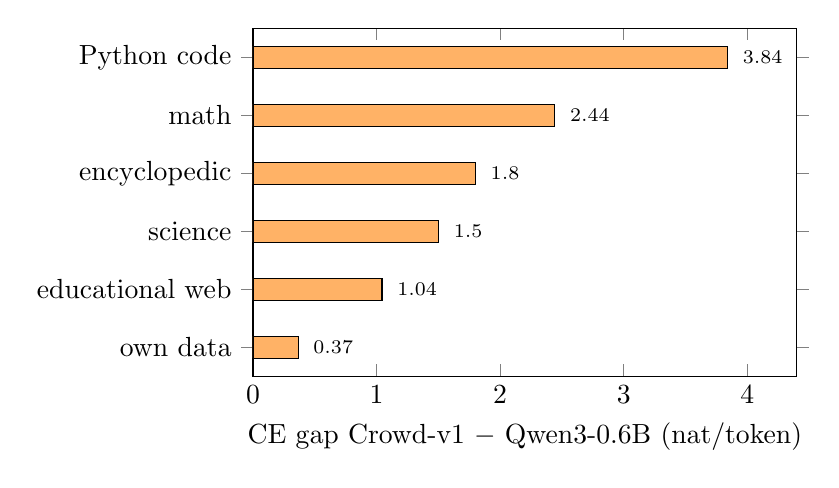
\begin{tikzpicture}
\begin{axis}[xbar, bar width=8pt, width=0.7\linewidth, height=6cm, xmin=0, xmax=4.4,
  xlabel={CE gap Crowd-v1 $-$ Qwen3-0.6B (nat/token)},
  symbolic y coords={own data,educational web,science,encyclopedic,math,Python code}, ytick=data,
  nodes near coords, nodes near coords style={font=\scriptsize}, every node near coord/.append style={xshift=2pt}]
\addplot[fill=orange!60] coordinates {(0.365,own data) (1.044,educational web) (1.501,science) (1.800,encyclopedic)
  (2.442,math) (3.840,Python code)};
\end{axis}
\end{tikzpicture}
\caption{P0: per-domain held-out gap to Qwen3-0.6B (same tokenizer, 8 windows of 2{,}048 tokens per domain).}
\label{fig:p0}
\end{figure}

\section{Discussion}
\label{sec:disc}
\paragraph{Is the null result specific to Crowd-v1?} Not established. The paper's LoRA table on NL-RX-SYNTH (lr
$2\times10^{-5}$, $\lambda=1$, $k=1$, 5 runs) reports $21.09\pm1.90\to32.46\pm1.26$ at rank 64 \cite{huang2025llmjepa}.
LoRA rank therefore does not explain our null: our SFT (17.1\%) is close to theirs. The remaining differences are:
\begin{itemize}
\item a 10$\times$ larger learning rate;
\item $k=0$;
\item 3 instead of about 4 epochs;
\item the model itself. The paper evaluates instruction-tuned models only; Crowd-v1 is a base model with an engram table.
\end{itemize}
The collapse we observe (final-state cosine $\to1$ within a few hundred steps, with general-loss damage) is consistent
with the anisotropy of final hidden states \cite{ethayarajh2019contextual}. A large learning rate may reach this
shortcut faster.

\paragraph{A ready test (P2).} The paper's LoRA recipe (lr $2\times10^{-5}$, $\lambda=1$, $k=1$ with a reserved token, 4
epochs) applied to Qwen3-0.6B and to Crowd-v1, with paired seeds. The reading of all four outcomes was fixed in advance:
\begin{itemize}
\item a gain on both points to our recipe;
\item a gain on Qwen only points to the model;
\item no gain on either means the effect does not reproduce at this scale.
\end{itemize}
P2 is implemented but not yet run: the T4 is reserved for training.

\paragraph{Limitations.}
\begin{itemize}
\item One task, one adapter rank and one seed in the screen.
\item Compute-matched comparisons penalize JEPA's per-step cost by design.
\item The screen's loss-dropout arms drew their dropout decision from the data-order RNG, so their batches were not
paired with SFT's. This adds noise but no bias, and was fixed afterwards.
\item The Qwen3-0.6B checkpoint used as reference is post-trained.
\item No French data was measured.
\end{itemize}

\section{Improvement proposals}
\begin{enumerate}
\item \textbf{Data mix.} Add code, mathematics and reference text to the CrowdGPT corpus, after license review by the
maintainer. Track the per-domain gaps on every checkpoint with the released evaluation tool.
\item \textbf{Evaluation.} Keep the held-out loss check engram-aware, and bind the engram table in the signed receipt.
\item \textbf{JEPA, if pursued.} Do not wire it into the volunteer client yet. If used, start from $\lambda=0.1$ with loss
dropout 0.5 and stop-gradient (the best guard-passing variant). Run P2, then LoRA r512 on a 24\,GB GPU, where the paper
reports its largest LoRA gain.
\item \textbf{Other models.} The natural pairs of views for other project models (docstring $\leftrightarrow$ code,
question $\leftrightarrow$ answer, statement $\leftrightarrow$ proof) are listed with a gate: nothing is built unless P2
shows a JEPA gain on Qwen3-0.6B.
\end{enumerate}

\section*{Reproducibility}
Code, protocols written before the runs, and raw results are in the HiveMind repository:
\begin{itemize}
\item code and protocols: \texttt{scripts/crowdgpt\_t4/};
\item raw results: \texttt{artifacts/experiments/CROWDGPT\_*};
\item reports: \texttt{docs/CROWDGPT\_LLM\_JEPA\_RESULTS.md} and \texttt{docs/CROWDGPT\_LLM\_JEPA\_STUDY.md}.
\end{itemize}
The opt-in loss module (\texttt{crowd\_jepa.py}), the per-domain evaluation tool and the data-mix proposal are proposed
to the CrowdGPT repository. Model weights and data are pinned by revision.

\section*{Acknowledgments}
We thank the CrowdGPT maintainer and its volunteer contributors for the open model and data. Experiment code, runs and
the first draft of this report were produced with an AI coding assistant (Claude, Anthropic) under the author's
direction. Every number was checked against the stored result files.

\begin{thebibliography}{99}
\bibitem{huang2025llmjepa} H.~Huang, Y.~LeCun, R.~Balestriero. LLM-JEPA: Large Language Models Meet Joint Embedding
Predictive Architectures. arXiv:2509.14252, 2025.
\bibitem{karpathy2026autoresearch} A.~Karpathy. autoresearch. \url{https://github.com/karpathy/autoresearch}, 2026.
\bibitem{lecun2022path} Y.~LeCun. A Path Towards Autonomous Machine Intelligence. OpenReview, 2022.
\bibitem{assran2023ijepa} M.~Assran et al. Self-Supervised Learning from Images with a Joint-Embedding Predictive
Architecture. CVPR, 2023.
\bibitem{grill2020byol} J.-B.~Grill et al. Bootstrap Your Own Latent: A New Approach to Self-Supervised Learning.
NeurIPS, 2020.
\bibitem{oord2018cpc} A.~van den Oord, Y.~Li, O.~Vinyals. Representation Learning with Contrastive Predictive Coding.
arXiv:1807.03748, 2018.
\bibitem{bardes2022vicreg} A.~Bardes, J.~Ponce, Y.~LeCun. VICReg: Variance-Invariance-Covariance Regularization for
Self-Supervised Learning. ICLR, 2022.
\bibitem{ethayarajh2019contextual} K.~Ethayarajh. How Contextual are Contextualized Word Representations? EMNLP, 2019.
\bibitem{hu2022lora} E.~J.~Hu et al. LoRA: Low-Rank Adaptation of Large Language Models. ICLR, 2022.
\bibitem{locascio2016nlrx} N.~Locascio, K.~Narasimhan, E.~DeLeon, N.~Kushman, R.~Barzilay. Neural Generation of Regular
Expressions from Natural Language with Minimal Domain Knowledge. EMNLP, 2016. arXiv:1608.03000.
\bibitem{douglas2023diloco} A.~Douillard et al. DiLoCo: Distributed Low-Communication Training of Language Models.
arXiv:2311.08105, 2023.
\bibitem{qwen3report} Qwen Team. Qwen3 Technical Report. arXiv:2505.09388, 2025.
\bibitem{crowdgpt} CrowdGPT. \url{https://github.com/Vxtzq/CrowdGPT}; model \url{https://huggingface.co/Vxtzq/Crowd-v1}.
\end{thebibliography}
\end{document}
